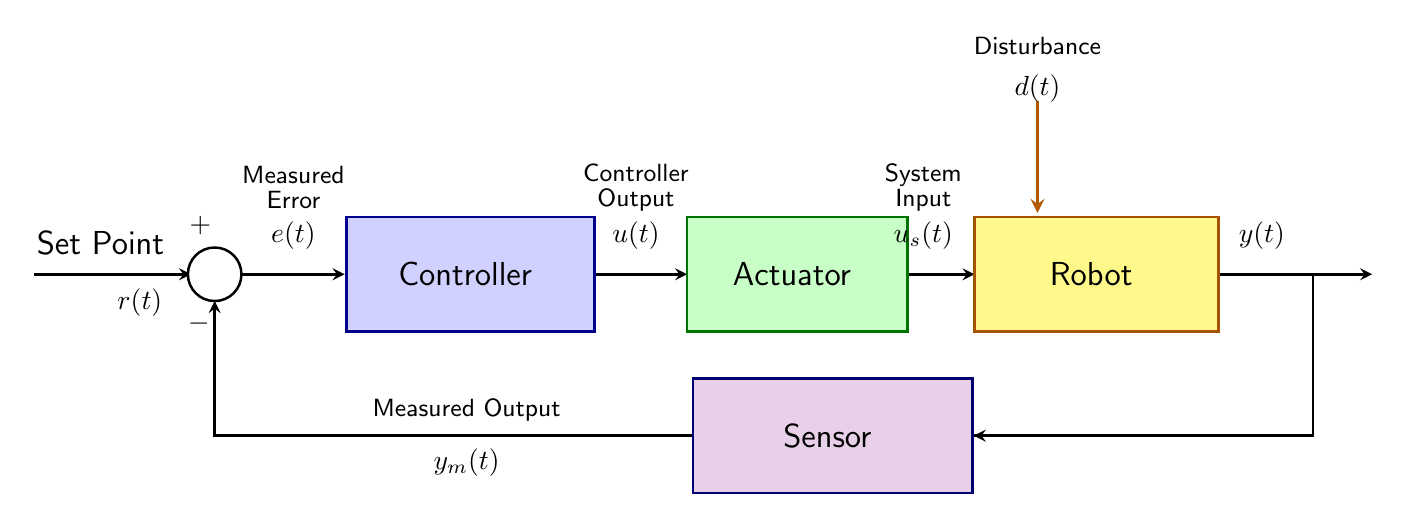
\begin{tikzpicture}[
   font=\sffamily,
   >=stealth,
   line width=0.9pt,
   block/.style={
      draw,
      minimum height=1.45cm,
      align=center,
      font=\sffamily\large
   }
]

   % Set point
   \draw[->] (-4.3,0) -- (-2.3,0);

   \node[above] at (-3.45,0.12) {\large Set Point};
   \node[below] at (-2.95,-0.05) {$r(t)$};

   % Summing junction
   \draw[fill=white] (-2,0) circle (0.34);

   \node at (-2.18,0.62) {$+$};
   \node at (-2.20,-0.63) {$-$};

   % Error signal
   \draw[->] (-1.66,0) -- (-0.35,0);

   \node[above] at (-1.00,0.18) {$e(t)$};

   \node[align=center] at (-1.00,1.10)
   {
      \small Measured\\[-1mm]
      \small Error
   };

   % Controller
   \node[
      block,
      fill=blue!18,
      draw=blue!55!black,
      minimum width=3.15cm
   ] (controller) at (1.25,0)
   {
      Controller
   };

   % Controller output
   \draw[->] (controller.east) -- (4.00,0);

   \node[above] at (3.35,0.18) {$u(t)$};

   \node[align=center] at (3.35,1.10)
   {
      \small Controller\\[-1mm]
      \small Output
   };

   % Actuator
   \node[
      block,
      fill=green!22,
      draw=green!45!black,
      minimum width=2.80cm
   ] (actuator) at (5.40,0)
   {
      Actuator
   };

   % System input
   \draw[->] (actuator.east) -- (7.65,0);

   \node[above] at (7.00,0.18) {$u_s(t)$};

   \node[align=center] at (7.00,1.10)
   {
      \small System\\[-1mm]
      \small Input
   };

   % Robot
   \node[
      block,
      fill=yellow!45,
      draw=orange!65!black,
      minimum width=3.10cm
   ] (robot) at (9.20,0)
   {
      Robot
   };

   % Robot output
   \draw[->] (robot.east) -- (12.70,0);

   \node[above] at (11.30,0.18) {$y(t)$};

   % Disturbance
   \draw[->,orange!70!black,line width=1.2pt]
      (8.45,2.20) -- (8.45,0.78);

   \node[align=center] at (8.45,2.60)
   {
      \small Disturbance\\[1mm]
      $d(t)$
   };

   % Sensor
   \node[
      block,
      fill=violet!18,
      draw=blue!45!black,
      minimum width=3.55cm
   ] (sensor) at (5.85,-2.05)
   {
      Sensor
   };

   % Output feedback to sensor
   \draw
      (11.95,0)
      -- (11.95,-2.05)
      -- (sensor.east);

   \draw[->]
      (11.95,-2.05)
      -- (sensor.east);

   % Sensor feedback to summing junction
   \draw[->]
      (sensor.west)
      -- (-2,-2.05)
      -- (-2,-0.34);

   \node[above] at (1.20,-2.00)
   {
      \small Measured Output
   };

   \node[below] at (1.20,-2.08)
   {
      $y_m(t)$
   };

\end{tikzpicture}